\documentclass[10pt,a4paper]{report}
%\usepackage[latin1]{inputenc}
\usepackage[utf8]{inputenc}
\usepackage{amsmath}
\usepackage{amsfonts}
\usepackage{amssymb}
\usepackage{graphicx}
\usepackage{multicol}
\usepackage{tabularx}
\usepackage{tikz}
\usetikzlibrary{arrows,shapes,automata,petri,positioning,calc}
\usepackage{hyperref}
\usepackage{tikz}
\usetikzlibrary{matrix,calc}
\usepackage[margin=0.5in]{geometry}
% ---- power functions -----% 
\newcommand{\myvec}[1]{\ensuremath{\begin{pmatrix}#1\end{pmatrix}}}
\let\vec\mathbf

\providecommand{\norm}[1]{\left\lVert#1\right\rVert}
\providecommand{\abs}[1]{\left\vert#1\right\vert}
\let\vec\mathbf

\newcommand{\mydet}[1]{\ensuremath{\begin{vmatrix}#1\end{vmatrix}}}
\providecommand{\brak}[1]{\ensuremath{\left(#1\right)}}
\providecommand{\lbrak}[1]{\ensuremath{\left(#1\right.}}
\providecommand{\rbrak}[1]{\ensuremath{\left.#1\right)}}
\providecommand{\sbrak}[1]{\ensuremath{{}\left[#1\right]}}
%-------end power functions----%
\newenvironment{Figure}
  {\par\medskip\noindent\minipage{\linewidth}}
  {\endminipage\par\medskip}
\begin{document}
%--------------------logo figure-------------------------%
\begin{figure*}[!tbp]
  \centering
  \begin{minipage}[b]{0.4\textwidth}
  
\includegraphics[scale=.25]{iitlogo.png} 
  \end{minipage}\vspace{0.2cm}
\end{figure*}
%--------------------name & rollno-----------------------
\raggedright \textbf{Name}:\hspace{1mm} GANGA GOPINATH\hspace{3cm} \Large \textbf{ Assignment}\hspace{2.5cm} % 
\normalsize \textbf{Roll No.} :\hspace{1mm} FWC22050\vspace{1cm}
\begin{multicols}{2}

%----------------problem statement--------------%
\raggedright \textbf{Problem Statement:}\vspace{2mm}
\raggedright \\Consider a family of circles which are passing through the point (-1, 1) and are tangent to x-axis. If (h, k) are the coordinates of the center of the circles, then the set of values of k is given by interval.\\
\vspace{5mm}
%-----------------------------solution---------------------------
\raggedright \textbf{SOLUTION}:\vspace{2mm}\\

%---------given----------------%
\raggedright \textbf{Given}:\vspace{2mm}\\
$\vec{O}$ be the center of circle and the coordinates are,\vspace{1mm}
\begin{align}
\vec{O}=\myvec{
h\\
k
}
\end{align}
 \vspace{2mm}
Let $\vec{X}$ be the point on the circle \\\vspace{1mm}
\begin{align}
    \vec{X} = \myvec{
    -1\\
    1
    }
\end{align}
%-------------To find ------------------%
\textbf{To Find }\vspace{2mm}\\
Constructing the family of circles with different values of k \vspace{2mm}  \\ 
%--------------steps----------------------%
\textbf{STEP-1}\vspace{2mm}\\
The perpendicular distance of center from tangent of the circle is equal to its radius.
Let r be the radius of circles   \\ \vspace{1mm}
%Let $\vec{O}$ be the center of circle and the coordinates are,\vspace{1mm}
%\begin{align}
%\vec{O}=\myvec{
%\gamma\\
%\beta
%}

So that r=k \\
Let $\vec{R}$ be the any point on the circle \\\vspace{1mm}
\begin{align}
    \vec{R} = &r \myvec{
    cos\theta\\
    sin\theta
    }
\end{align}
For the input parameters in Table 1.\\
{\setlength\extrarowheight{2pt}
\begin{center}
\begin{tabular}{|c|c|c|}
	\hline
	\textbf{Symbol}&\textbf{Value}&\textbf{Description}\\
	\hline
O&$\begin{pmatrix}
	\gamma\\
	\alpha\\
	\end{pmatrix} $& Center\\
	\hline
	X&$\begin{pmatrix}
	-1\\1\\
	\end{pmatrix} $& Passing point\\
	\hline
	R& r \myvec{
    cos\theta\\
    sin\theta }
     & point on circle\\
	\hline
	r &$\alpha$  & radius\\
	\hline
\end{tabular}
%}\\
\\ {Table 1}\\
\end{center}
\vspace{3mm} 


\textbf{STEP-2}\vspace{2mm}\\
%The equation of circle is given by, \\ \vspace{1mm}
The distance between the point $\vec{X}$ and $\vec{O}$ is given by, \\ \vspace{1mm}
\begin{align}
    \norm{\vec{X}-\vec{O}} = r 
\end{align}
\vspace{2mm}
which can be expressed as
\begin{center}
   $ \sqrt{(\vec{X}-\vec{O})^{\top}(\vec{X}-\vec{O})} = r $
\end{center}\vspace{5mm}

Squaring on both the sides \\ \vspace{2mm}
\begin{center}
( $ \sqrt{(\vec{X}-\vec{O})^{\top}(\vec{X}-\vec{O})} )^2 = r^2 $\\ \vspace{0.5cm}
$(\vec{X}-\vec{O})^{\top}(\vec{X}-\vec{O})=r^2$
\end{center}
Expanding the above equation,\\ \vspace{1mm}
\begin{align}
    \norm{\vec{X}}^2-2\vec{X}^{\top}\vec{O}+\norm{\vec{O}}^2=r^2
\end{align}
Upon substituting numerical values,
\begin{equation}
 (-1)^2+1^2-2 \myvec{-1 \\ 1}^{\top}\myvec{ \gamma \\ \alpha}+ \gamma^2 +\alpha^2 =\alpha^2 
 \end{equation}
 \begin{equation} 
 (-1)^2+1^2-2 \myvec{-1 & 1} \myvec{ \gamma \\ \alpha}+ \gamma^2 +\alpha^2 =\alpha^2 
 \end{equation}
 \begin{equation}
 2+2 \gamma-2\alpha+\gamma^2=0
 \end{equation}
Solving the above equation ,
\begin{equation}
\alpha \geq \frac{1}{2}
\end{equation}
Let $\alpha$ be any value from $\frac{1}{2}$ to $\infty$\\ \vspace{1mm}
\begin{align}
    \alpha \in [\frac{1}{2},\infty)
\end{align}
%\textbf{STEP-3}\vspace{2mm}\\
%The point of contact $\vec{B}$, the equation of a tangent  is 
 % \begin{align}
  %\brak{\vec{V}\vec{q}+\vec{u}}^{\top}\vec{x}+\vec{u}^{\top}\vec{q}+f = 0
  %\end{align}
%where  
 % \begin{align}
  %         \vec{V} &= \myvec{1 & 0\\ 0 & 1},\\
   %   \vec{u} &= \myvec{{\gamma} \\ {\alpha}},\\
    %  \vec{q} &= \myvec{{\gamma} \\ 0},\\
     % \vec{X} &= \myvec{-1 \\ 1},\\ 
     %f={\gamma}^2+{\alpha}^2-r^2     
    %\end{align}
%After substituting,
%\begin{align}
%\begin{multline}
%\myvec{\myvec{ 1 & 0\\ 0&1}\myvec{\gamma\\0}+\myvec{\gamma \\ \alpha}}^{\top}\myvec{-1 %\\ 1}+\\ 
 %\myvec{ \gamma \\ \alpha}^\top\myvec{ \gamma \\ 0}+ \gamma^2+\alpha^2-r^2=0 \\ 
%\end{multline}
%\begin{multline}
%\myvec{\myvec{\gamma\\0}+\myvec{\gamma \\ \alpha}}^{\top}\myvec{-1 \\ 1}+ \\
 %\myvec{ \gamma & \alpha}\myvec{ \gamma \\ 0}+ \gamma^2+\alpha^2-\alpha^2=0 \\
%\end{multline}
%\end{align}
which can be expressed as,
%\begin{align}
%2{\gamma}^2-2\gamma+\alpha=0
%\end{align}

Let $\theta$ be any angle from 0 to 2$\pi$\\ \vspace{1mm}
\begin{align}
    \theta \in [0,2\pi)
\end{align}
Let us assume, \\ \vspace{1mm}
\begin{align}
    \theta=\frac{\pi}{3} 
\end{align}
Using equation (3) any point on circle   $ \vec{R}=\myvec{
    x\\
    y
    } $ is, \\ \vspace{1mm}
    Here ,\\  \vspace{2mm}
\begin{align}
    x=rcos\theta\\
    y=rsin\theta
\end{align}
\begin{align}
 \vec{R}=\myvec{
    0.5\\
    .86
    } 
\end{align}
Let $\alpha$ be any values ranging from $\frac{1}{2}$ to $\infty$  with the incrementation of +2\\
So, \\ 
\begin{align}
    \alpha = 1,3,5,7,9,11
\end{align}
If $\alpha=1$ ,\\ 
\begin{align}
    \vec{O}=\myvec{
    0\\
    1
    }
\end{align}
when $\alpha=3$ and so on till $\alpha=11$,\\ 
\begin{align}
    \vec{O}=\myvec{
    1.23\\
   3
    } 
\end{align}
\begin{center}
 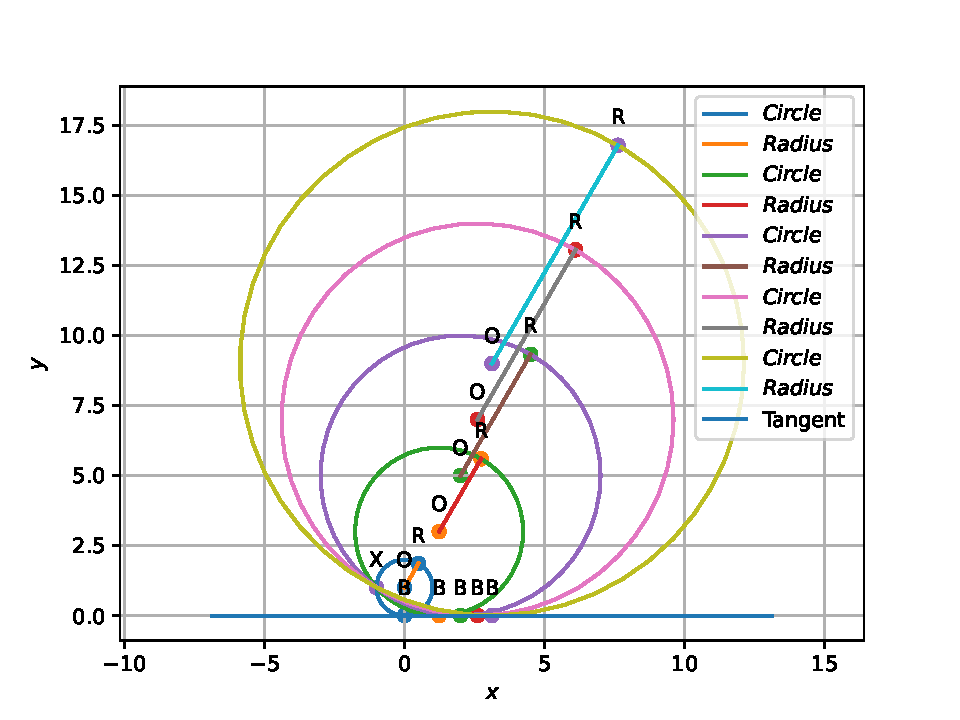
\includegraphics[width=0.5\textwidth]{circle.pdf}  
 \end{center}\vspace{1mm}
 \vspace{2mm} \textbf{Construction}
\begin{center}
\setlength{\arrayrulewidth}{0.5mm}
\setlength{\tabcolsep}{6pt}
\renewcommand{\arraystretch}{1.5}
    \begin{tabular}{|l|c|}
    \hline 
    \textbf{vertex} & \textbf{coordinates} \\ \hline
   $\vec{O}$ & $\myvec{
   \gamma\\
   \alpha
   } $ \\\hline
   $\vec{X}$ & $\myvec{
   -1\\
   1
   } $ \\\hline
      \end{tabular}
  \end{center}
  

\raggedright  Download the code \\
https://github.com/Gangagopinath/ASSIGNMENT/tree/
\newline
main/assignment5
}  \end{multicols}
\end{document}
